% !TeX root = ../main.tex

\chapter{相关技术概述}

...

本章主要对其中涉及的基本概念与相关技术进行介绍。

\section{西瓜种植}

...
虽然西瓜很好吃,但我不喜欢有很多种子的。

\subsection{西瓜种子的最大公约数}

所以只能边吃西瓜边数种子。
展示一下可以写伪代码,说实话感觉格式优点麻烦。
譬如辗转相除法伪代码示例如下:

\begin{algorithm}
  \caption{辗转相除法}
  \label{alg1}
  \small
  \begin{algorithmic}
    \WHILE{$b \neq 0$}
      \IF{$a \ge b$}
        \STATE $a \leftarrow a - b$
      \ELSE
        \STATE $b \leftarrow b - a$
      \ENDIF
    \ENDWHILE
  \end{algorithmic}
\end{algorithm}




\section{鸡鸭养殖}

鸡鸭适合养在树林里,这样既可以节约空间,鸡也可以找虫子吃,粪便还可作为肥料,旁边要是再有个小池塘就更好了。

\subsection{循环生态的应用}


% TIKZ 画自动机

FSM 逻辑如图~\ref{fig:fsm-logic-example} 所示,它的输入和当前状态决定着下一个状态和输出。

\begin{figure}[htb]
  \centering
  \begin{tikzpicture}[node distance=12pt]
    \node[draw, rounded corners]                        (start)   {输入};
    \node[draw, below right=10pt of start]                         (transition)  {状态转移条件};
    \node[draw, aspect=2, below=60pt of start]     (output conditions)  {输出条件};
    \node[draw, below=of transition]                        (state)  {状态};
    \node[draw, rounded corners, below=of output conditions]  (end)     {输出};
    \coordinate[right=40pt of state] (point1);
    
    \draw[->] (start)  |- (transition);
    \draw[->] (transition) -- (state);
    \draw[->] (state) |-  (output conditions);
    \draw[->] (output conditions) -- (end);
    \draw[->] (start)  -- (output conditions);
    \draw[->] (state)  -- (point1)  |-  (transition);
  \end{tikzpicture}
  \caption{FSM 逻辑示意图} \label{fig:fsm-logic-example}
\end{figure}




\subsection{确定有限状态机}

通常使用没有起点的箭头表示开始状态,双圆圈表示接受状态。
自动机中开始状态也可以是接受状态,此时表示其接受空字符串。

如图 \ref{fig:fsm-binary-even-zero-example} 所示,这是一台用于判断输入二进制字符串是否含有偶数个 0 的有限自动机的逻辑图。
$S_1$ 为开始状态,并代表已经输入了偶数个 0,因此 $S_1$ 也是接受状态。
若输入为不包含 0 或含有偶数个 0 的字符串(例如:1,100,01011等),则自动机以接受状态结束。

\begin{figure}[htb]
  \centering
    \begin{tikzpicture}[shorten >=1pt,auto,transform shape]
    \node[initial,state, accepting] (s1) {$S_1$};
    \node[state] (s2) [right of=s1]  {$S_2$};
    \path[->] (s1) edge [bend left] node [align=center]  {0} (s2)
          (s1) edge [loop above]      node [align=center]  {1} (s1)
          (s2) edge [bend left]       node [align=center]  {0} (s1)
          (s2) edge [loop right]       node [align=center]  {1} (s2);
    \end{tikzpicture}
  \caption{FSM:检测二进制数是否含有偶数个零}
  \label{fig:fsm-binary-even-zero-example}
\end{figure}

同时它也是一个确定有限状态机(DFA),对字母表中每个符号,确定有限自动机的状态都有且仅有一个转移。
它对应的状态转移表如表~\ref{tab:fsm-state-example} 所示:

\begin{table}
  \centering
  \caption{状态转移表}
  \begin{tabular}{c|ccc}
    \toprule
    输入状态 & 1 & 0   \\
    \midrule
    $S_1$   & $S_1$ & $S_2$  \\
    $S_2$   & $S_2$ & $S_1$  \\
    \bottomrule
  \end{tabular}
  \label{tab:fsm-state-example}
\end{table}


\section{虚拟世界}

...

\subsection{坐标系}

还可以用 TIKZ 画坐标系。

目前工业界的各类软件采用坐标系也各不相同,
譬如 Unreal、Unity、Babylon、DirectX 均采用左手坐标系(如图~\ref{fig:left-hand-coordinate-system}),
而 Three.js、Cocos、OpenGL、Vulkan 等则采用右手坐标系(如图~\ref{fig:right-hand-coordinate-system})。

\begin{figure}[htb]
  \centering
  \begin{minipage}[t]{.4\textwidth}
    \centering
    \begin{tikzpicture}[x=0.5cm, y=0.5cm, z=0.3cm]
      % Axes
      \draw [->] (0,0,0) -- (4,0,0) node [at end, right] {$X$};
      \draw [->] (0,0,0) -- (0,4,0) node [at end, left] {$Y$};
      \draw [->] (0,0,0) -- (0,0,4) node [at end, left] {$Z$};
    \end{tikzpicture}
    \caption{左手坐标系}
    \label{fig:left-hand-coordinate-system}
  \end{minipage}
  \begin{minipage}[t]{.4\textwidth}
    \centering
    \begin{tikzpicture}[x=0.5cm, y=0.5cm, z=-0.3cm]
      % Axes
      \draw [->] (0,0,0) -- (4,0,0) node [at end, right] {$X$};
      \draw [->] (0,0,0) -- (0,4,0) node [at end, left] {$Y$};
      \draw [->] (0,0,0) -- (0,0,4) node [at end, left] {$Z$};
    \end{tikzpicture}
    \caption{右手坐标系}
    \label{fig:right-hand-coordinate-system}
  \end{minipage}
\end{figure}


\section{数学公式}

\subsection{四元数的定义}

譬如四元数:

\begin{equation}
  i^2 = j^2 = k^2 = -1 \\
\end{equation}
\begin{equation}
\begin{aligned}
  ij = -ji = k \\
  ki = -ik = j \\
  jk = -kj = i
\end{aligned}
\end{equation}


\subsection{四元数的几何意义}

TIKZ 画坐标系。

在平面坐标系上,以横坐标 R 代表实部,纵坐标 I 代表虚部,复数的几何意义如图~\ref{fig:complex-number}。

\begin{figure}[htb]
  \centering
    \begin{tikzpicture}
      \coordinate (origin) at (0,0);
      \coordinate (ab) at (2,1);
      \coordinate (ba) at (-1,2);

      \draw[-stealth] (-2.5,0) -- (2.5,0) node[right](r) {$R$}; 
      \draw[-stealth] (0,-1) -- (0,2.5) node[right](i) {$I$}; 

      \draw [->, thick] (origin) -- (ab) node[at end, right]{$a+bi$};
      \draw [->, thick] (origin) -- (ba) node[at end, left]{$-b+ai$};
      
      \draw [loosely dashed] (0,1) node[left]{$bi$} -- (ab);
      \draw [loosely dashed] (2,0) node[below]{$a$} -- (ab);

      \draw [loosely dashed] (-1,0) node[below]{$-b$} -- (ba);
      \draw [loosely dashed] (0,2) node[right]{$ai$} -- (ba);

      \pic [draw, -, "$\theta$",angle radius=4pt , angle eccentricity=2] {right angle = ab--origin--ba};
      \pic [draw=red, ->, angle radius=2.23cm, angle eccentricity=2] {angle = ab--origin--ba};
    \end{tikzpicture}
  \caption{复数的几何意义}
  \label{fig:complex-number}
\end{figure}
$(a+bi)*i=-b+ai$,复数乘以 $i$,相当于将平面上复数做逆时针旋转 $\theta$($90^{\circ}$)。

同理非零四元数通常可用于描述三维空间的拉伸与旋转变换,单位 $i$、$j$、$k$ 的几何意义则可以理解为三维空间的一种旋转。
以右手坐标系(如图~\ref{fig:right-hand-coordinate-system})为例,
其中 $i$ 代表绕 $Z$ 轴($X$正向向$Y$轴正向)旋转,$j$ 代表绕 $Y$ 轴($Z$正向向$X$轴正向)旋转,$k$ 代表绕 $X$ 轴($Y$正向向$Z$轴正向)旋转。

四元数模长定义如公式\eqref{eq:quaternion-norm},当 $q=a+bi+cj+dk$,$||q||=1$ 时,它所代表的变换并不会对原向量进行缩放,而是一个纯旋转。
\begin{equation}
  ||q|| = a^2 + b^2 + c^2 + d^2
  \label{eq:quaternion-norm}
\end{equation}

此时 $q$ 被称为单位四元数,也因此它通常被用于表示三维空间的旋转。
同时四元数在静态坐标系中的代数计算,使其避免了动态欧拉角所造成的万向锁问题。

\subsection{四元数的其他优势}

四元数相比旋转矩阵与欧拉角,除了可以避免万向锁问题,还具有其他方面的优势。
譬如速度更快、占用存储空间小、更易于平滑插值等。

3D 空间中任意一个旋转都能够使用三个四元数相乘的形式进行表达,即 $ R_{q}(p) = qpq^{-1} $,其中 $q$ 为一个单位四元数,$p$ 为一个纯四元数。
$ R_{q} $ 表示一个可以将空间点 $p$ 旋转到空间另一个点 $ R_{q}(p) $ 的一个旋转。

定义一个四元数 $ q=a+bi+cj+dk $ 的共轭为 $ q^* = a - bi -cj -dk $。

设 $ \mathbf{v} = bi+cj+dk $,则 $ q=[s,\mathbf{v}] $,$ q^*=[s,-\mathbf{v}] $,此时:
\begin{equation}
qq* = s^2 + v^2 = ||q||^2
\end{equation}

由于 $q^{-1}=\frac{q^*}{||q||^2} $,若使用单位四元数,则模长($ ||q||^2 $)为 1,故此时:
\begin{equation}
q^{-1} = \frac{q^*}{1} = q^*
\end{equation}

存在 3D 旋转公式,任意向量 $\mathbf{v}$ 沿着以单位向量定义的旋转轴 $\mathbf{u}$ 旋转 $\theta$ 度之后的 $\mathbf{v}^{'}$ 可以使用四元数乘法获得。
令 $v=[0,\mathbf{v}]$,$q=[\cos{\frac{1}{2}\theta},\sin{\frac{1}{2}\theta}\mathbf{u}]$,则:
\begin{equation}
v^{'} = qvq^{-1} = qvq^*
\end{equation}

同时存在与单位四元数旋转效果相同的 3D 旋转矩阵,即任意向量 $\mathbf{v}$ 沿着以单位向量定义的旋转轴 $\mathbf{u}$ 旋转 $\theta$ 角度之后的 $\mathbf{v}^{'}$ 可以使用矩阵乘法来获得。

令 $a=\cos{\frac{1}{2}\theta}$,$b=\sin{\frac{1}{2}\theta}u_x$,$c=\sin{\frac{1}{2}\theta}u_y$,$d=\sin{\frac{1}{2}\theta}u_z$,那么:
\begin{equation}
  \mathbf{v}^{'} = 
  \begin{bmatrix}
    1-2c^2-2d^2 & 2bc-2ad & 2ac+2bd \\
    2bc+2ad & 1-2b^2-2d^2 & 2cd-2ab \\
    2bd-2ac & 2ab+2cd & 1-2b^2-2c^2 \\
  \end{bmatrix}
  \mathbf{v}
\end{equation}

由上可知,四元数相对于旋转矩阵,使用 $q^*$ 替换 $q^{-1}$,大大提高了求四元数的逆的计算效率,同时比旋转矩阵的计算更为快速方便。
此外,四元数对应实部与虚部 $ijk$ 只需要存储四个数值,空间占用也远小于同等效果的旋转矩阵。

\subsubsection{绘制箭头示例}

线性插值(Lerp)会沿一条直线进行插值,如图 \ref{fig:lerp} 所示,$v_t$ 在 $v_0$ 与 $v_1$ 组成的三角形斜边上滑动。

\begin{figure}[htb]
  \centering
  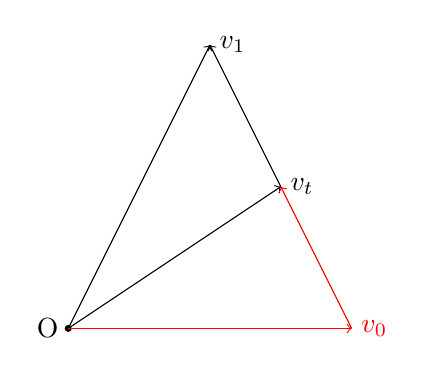
\begin{tikzpicture}[scale=0.9]
    \coordinate (o) at (0,0);
    \coordinate (v1) at (2,4);
    \coordinate (vt) at (3,2);
    \coordinate (v0) at (4,0);
    
    \fill[black] (o) circle (0.05) node[left]{O};
    
    \draw[->] (o) -> (v1) node[right]{$v_1$};
    \draw[->] (o) -> (vt) node[right]{$v_t$};
    \draw[red, ->] (o) -> (v0) node[right]{$v_0$};
    \draw[red, ->] (v0) -> (vt);
    \draw[->] (vt) -> (v1);
  \end{tikzpicture}
  \caption{线性插值示意图}
  \label{fig:lerp}
\end{figure}

$v_t$ 可写为 $v_0 + (v_1-v_0)t$,其中 $t$ 是插值的参数,取值范围为 $[0,1]$。
\begin{equation}
  v_t = Lerp(v_0, v_1,t) = v_0 + (v_1-v_0)t = (1-t)v_0+tv_1
\end{equation}

将 Lerp 应用于单位四元数上,可得:
\begin{equation}
  q_t = Lerp(q_0, q_1, t) = (1-t)q_0 + tq_1
  \label{eq:quaternions-lerp}
\end{equation}

\subsection{贝塞尔曲线}

贝塞尔曲线最初由 Paul de Casteljau 使用 de Casteljau 算法开发,是一种计算曲线的稳定方法。
其根据控制点的数量可分为不同阶,常见类型有线性贝塞尔曲线、二次贝塞尔曲线(也曾被用于 TrueType 的字体平滑)、三次贝塞尔曲线等。

线性贝塞尔曲线等同于线性插值,给定两个控制点 $P_0$ 与 $P_1$,则公式为:
\begin{equation}
  {\mathbf  {B}}(t)={\mathbf  {P}}_{0}+({\mathbf  {P}}_{1}-{\mathbf  {P}}_{0})t=(1-t){\mathbf  {P}}_{0}+t{\mathbf  {P}}_{1}{\mbox{ , }}t\in [0,1]
\end{equation}

二次贝塞尔曲线给定三个点 $P_1$、$P_2$ 与 $P_3$,公式为:
\begin{equation}
  {\mathbf  {B}}(t)=(1-t)^{{2}}{\mathbf  {P}}_{0}+2t(1-t){\mathbf  {P}}_{1}+t^{{2}}{\mathbf  {P}}_{2}{\mbox{ , }}t\in [0,1]
\end{equation}

三次贝塞尔曲线如图~\ref{fig:bezier-curve-3rd} 所示,给定四个点 $P_1$、$P_2$、$P_3$ 与 $P_4$,公式为:
\begin{equation}
  {\mathbf  {B}}(t)={\mathbf  {P}}_{0}(1-t)^{3}+3{\mathbf  {P}}_{1}t(1-t)^{2}+3{\mathbf  {P}}_{2}t^{2}(1-t)+{\mathbf  {P}}_{3}t^{3}{\mbox{ , }}t\in [0,1]
\end{equation}

\begin{figure}[htb]
  \centering
  \begin{tikzpicture}[scale=1.3]
    \coordinate (p0) at (0,0);
    \coordinate (p1) at (2,2);
    \coordinate (p2) at (4,2);
    \coordinate (p3) at (4,0);
    
    \fill[black] (p0) circle (0.05) node[left]{$P_0$};
    \fill[black] (p1) circle (0.05) node[above]{$P_1$};
    \fill[black] (p2) circle (0.05) node[above]{$P_2$};
    \fill[black] (p3) circle (0.05) node[right]{$P_3$};
    
    \draw[dashed] (p0) -> (p1);
    \draw[dashed] (p1) -> (p2);
    \draw[dashed] (p2) -> (p3);
  
    \draw (p0) .. controls (p1) and (p2) .. (p3);
  \end{tikzpicture}
  \caption{三次贝塞尔曲线}
  \label{fig:bezier-curve-3rd}
\end{figure}

$n$ 阶贝塞尔曲线给定 $P_0$、$P_1$、…、$P_n$ 等 $n+1$ 个点,公式可递归表达为:
\begin{equation}
  {\mathbf  {B}}(t)={\mathbf  {B}}_{{{\mathbf  {P}}_{0}{\mathbf  {P}}_{1}\ldots {\mathbf  {P}}_{n}}}(t)=(1-t){\mathbf  {B}}_{{{\mathbf  {P}}_{0}{\mathbf  {P}}_{1}\ldots {\mathbf  {P}}_{{n-1}}}}(t)+t{\mathbf  {B}}_{{{\mathbf  {P}}_{1}{\mathbf  {P}}_{2}\ldots {\mathbf  {P}}_{n}}}(t)
\end{equation}

De Casteljau 算法\cite{farin2000essentials}即基于此公式,采用递归方式来计算一组控制点所构建的贝塞尔曲线所经过的点。

给定 $P_0$ 到 $P_3$ 的控制点,将其分解为 $L_0L_1L_2L_3$ 与 $R_0R_1R_2R_3$ 继续绘制,并可通过级别控制绘制的精细度,
关键点如图~\ref{fig:de-casteljau} 所示:

\begin{figure}[htb]
  \centering
  \begin{tikzpicture}
    \coordinate (p0) at (0,0);
    \coordinate (p1) at (4,4);
    \coordinate (p2) at (8,4);
    \coordinate (p3) at (8,0);
    \coordinate (h) at (6,4);
    \coordinate (l0) at (0,0);
    \coordinate (l1) at (2,2);
    \coordinate (l2) at (4,3);
    \coordinate (l3) at (5.5,3);
    \coordinate (r0) at (5.5,3);
    \coordinate (r1) at (7,3);
    \coordinate (r2) at (8,2);
    \coordinate (r3) at (8,0);
    
    \fill[black] (h) circle (0.05) node[above]{$H$};
    
    \fill[black] (p0) circle (0.05) node[left]{$P_0$};
    \fill[black] (p1) circle (0.05) node[above]{$P_1$};
    \fill[black] (p2) circle (0.05) node[above]{$P_2$};
    \fill[black] (p3) circle (0.05) node[right]{$P_3$};
    
    \fill[black] (l0) circle (0.05) node[right]{$L_0$};
    \fill[black] (l1) circle (0.05) node[above]{$L_1$};
    \fill[black] (l2) circle (0.05) node[above]{$L_2$};
    \fill[black] (l3) circle (0.05) node[below right]{$L_3$};
    
    \fill[black] (r0) circle (0.05) node[below left]{$R_0$};
    \fill[black] (r1) circle (0.05) node[above]{$R_1$};
    \fill[black] (r2) circle (0.05) node[right]{$R_2$};
    \fill[black] (r3) circle (0.05) node[left]{$R_3$};
    
    \draw[-] (p0) -> (p1);
    \draw[-] (p1) -> (p2);
    \draw[-] (p2) -> (p3);
    
    \draw[red] (l1) -> (h);
    \draw[red] (h) -> (r2);
    \draw[blue] (l2) -> (r1);
  
  \end{tikzpicture}
  \caption{De Casteljau 算法绘制过程}
  \label{fig:de-casteljau}
\end{figure}

绘制 $P_0$ 到 $P_3$ 曲线的代码示例如下所示:

\begin{lstlisting}[language=python]
% 返回这两点间线段的中点
def midpoint((x1, y1), (x2, y2)):
    return ((x1+x2)/2, (y1+y2)/2)

% 绘制级别,可决定精细度
MAX_LEVEL = 5
def draw_curve(P0, P1, P2, P3, level=1):
    % 当级别达到最大时,则绘制两点之间直线
    if level == MAX_LEVEL:
        d.line((P0, P3))
    else:
        L0 = P0
        L1 = midpoint(P0, P1)
        H  = midpoint(P1, P2)
        R2 = midpoint(P2, P3)
        R3 = P3
        L2 = midpoint(L1, H)
        R1 = midpoint(R2, H)
        L3 = midpoint(L2, R1)
        R0 = L3
        % 绘制左半段贝塞尔曲线 L0-L1-L2-L3
        draw_curve(L0, L1, L2, L3, level+1)
        % 绘制右半段贝塞尔曲线 R0-R1-R2-R3
        draw_curve(R0, R1, R2, R3, level+1)

% 根据输入的点绘制曲线
draw_curve((10,10),(100,100),(100,10),(100,100))
\end{lstlisting}


\section{本章小结}

本章在第一节中介绍了...
在第二节中介绍了...
